\documentclass{article}
\usepackage{ctex}
\usepackage{fancyhdr}
\usepackage{extramarks}
\usepackage{amsmath}
\usepackage{amsthm}
\usepackage{amsfonts}
\usepackage{tikz}
\usepackage[plain]{algorithm}
\usepackage{algpseudocode}
\usepackage{extarrows}
\usepackage{indentfirst}

\usepackage[titletoc]{appendix}
\usepackage{pythonhighlight}
\usepackage{listings}
\usepackage[framed,numbered,autolinebreaks,useliterate]{mcode}

\usetikzlibrary{automata,positioning}

%
% Basic Document Settings
%

\topmargin=-0.45in
\evensidemargin=0in
\oddsidemargin=0in
\textwidth=6.5in
\textheight=9.0in
\headsep=0.25in

\linespread{1.1}

\pagestyle{fancy}
\lhead{\hmwkAuthorName}
\chead{\hmwkClass\ : \hmwkTitle}
\rhead{}
\lfoot{\lastxmark}
\cfoot{\thepage}

\renewcommand\headrulewidth{0.4pt}
\renewcommand\footrulewidth{0.4pt}

\setlength\parindent{2em}

%
% Create Problem Sections
%



\setcounter{secnumdepth}{0}
\newcounter{partCounter}
\newcounter{homeworkProblemCounter}
\setcounter{homeworkProblemCounter}{1}
\nobreak\extramarks{Problem \arabic{homeworkProblemCounter}}{}\nobreak{}

%
% Homework Problem Environment
%
% This environment takes an optional argument. When given, it will adjust the
% problem counter. This is useful for when the problems given for your
% assignment aren't sequential. See the last 3 problems of this template for an
% example.
%


%
% Homework Details
%   - Title
%   - Due date
%   - Class
%   - Section/Time
%   - Instructor
%   - Author
%

\newcommand{\hmwkTitle}{一元方程求解}
\newcommand{\hmwkDueDate}{March, 2022}
\newcommand{\hmwkClass}{数值分析作业}
\newcommand{\hmwkClassTime}{}
\newcommand{\hmwkClassInstructor}{}
\newcommand{\hmwkAuthorName}{\textbf{葛雨辰  201800150053}}

%
% Title Page
%

\title{
    \vspace{2in}
    \textmd{\textbf{\hmwkClass:\ \hmwkTitle}}\\
    \normalsize\vspace{0.1in}\small{Due\ on\ \hmwkDueDate\ }\\
    \vspace{0.1in}\large{\textit{\hmwkClassInstructor\ \hmwkClassTime}}
    \vspace{3in}
}

\author{\hmwkAuthorName}
\date{}

\renewcommand{\part}[1]{\textbf{\large Part \Alph{partCounter}}\stepcounter{partCounter}\\}

%
% Various Helper Commands
%

% Useful for algorithms
\newcommand{\alg}[1]{\textsc{\bfseries \footnotesize #1}}

% For derivatives
\newcommand{\deriv}[1]{\frac{\mathrm{d}}{\mathrm{d}x} (#1)}

% For partial derivatives
\newcommand{\pderiv}[2]{\frac{\partial}{\partial #1} (#2)}

% Integral dx
\newcommand{\dx}{\mathrm{d}x}

% Alias for the Solution section header
\newcommand{\solution}{\textbf{\large Solution}}

% Probability commands: Expectation, Variance, Covariance, Bias
\newcommand{\C}{\mathrm{C}}
\newcommand{\D}{\mathrm{D}}
\newcommand{\E}{\mathrm{E}}
\newcommand{\U}{\mathrm{U}}
\newcommand{\Z}{\mathbb{Z}}
\newcommand{\R}{\mathbb{R}}
\newcommand{\Q}{\mathbb{Q}}
\newcommand{\N}{\mathbb{N}}
\begin{document}

\maketitle

\pagebreak
\section{1. 序言}

本章节研究一元方程求根问题,依据2.2节的第三段话,我认为求根问题的算法分为\textbf{直接求根的算法}(二分法,牛顿法,割线法与试错法等)与\textbf{通过转化为不动点迭代间接求根的算法}(不动点迭代法,Aitken加速法,Steffensen迭代法等)。最后有关多项式有特殊的算法算法,涵盖Horner算法,及采取\textbf{嵌套方式}去计算多项式在固定点的值与导数值求多项式及导数的值,同时Muller求根算法可以很好地逼近复根。

首先声明以下所有程序都\textbf{按照方法名称命明},变量含义自明。

\section{2. 二分法,牛顿法,割线法与试位法对比}

\subsection{2.1 求解三阶Legendre方程在1.2附近的根}

考虑三阶的Legendre方程(作平移变换,方便误差估计)
    $$ P_3(x)=\frac{1}{2}\big[5(x-1)^3-3(x-1)\big]=0
    $$
    在1.2附近的根。观察在$[0,2]$上的方程曲线图像如下所示,我们很容易发现这个根的精确值$p=1$。
    \begin{figure}[h]
    \centering
    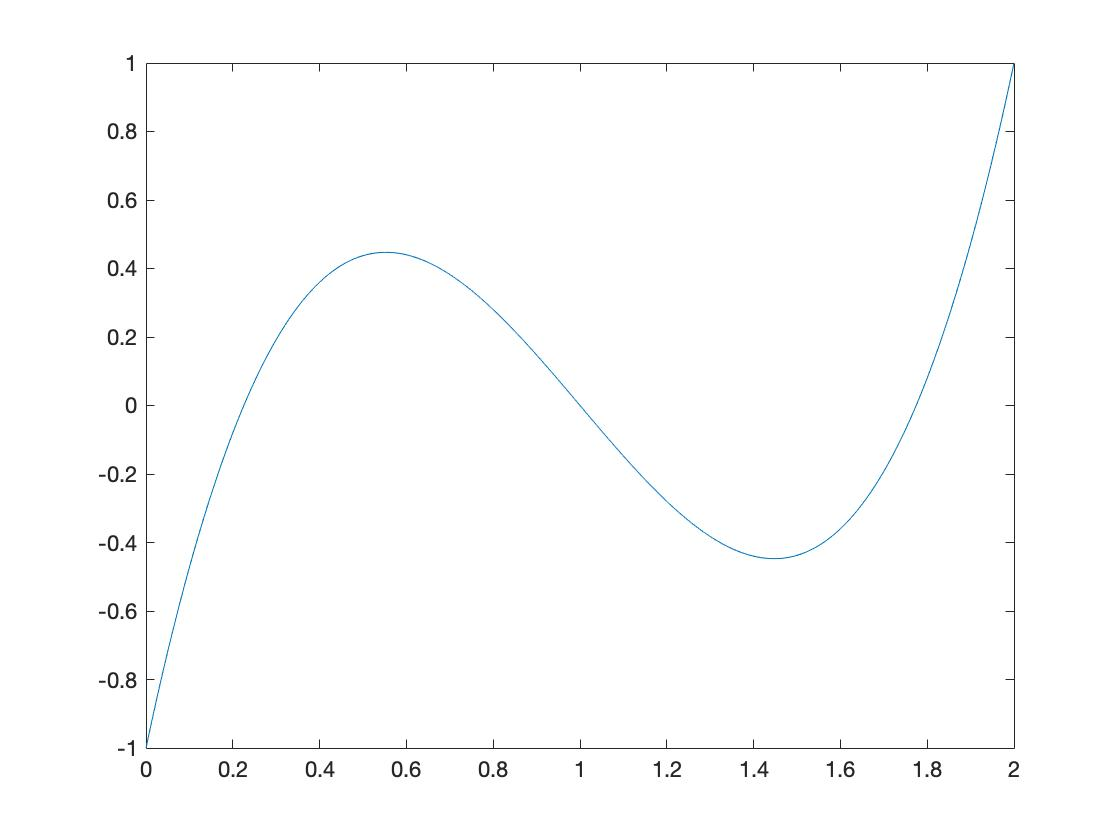
\includegraphics[scale=0.17]{Legendre.jpg}
    \caption{三阶的Legendre方程图像}
    \label{三阶的Legendre方程图像}
    \end{figure}

    下面分别运行二分法,牛顿法,割线法与试位法的程序,如下所示:
    \begin{figure}[h]
    \centering
    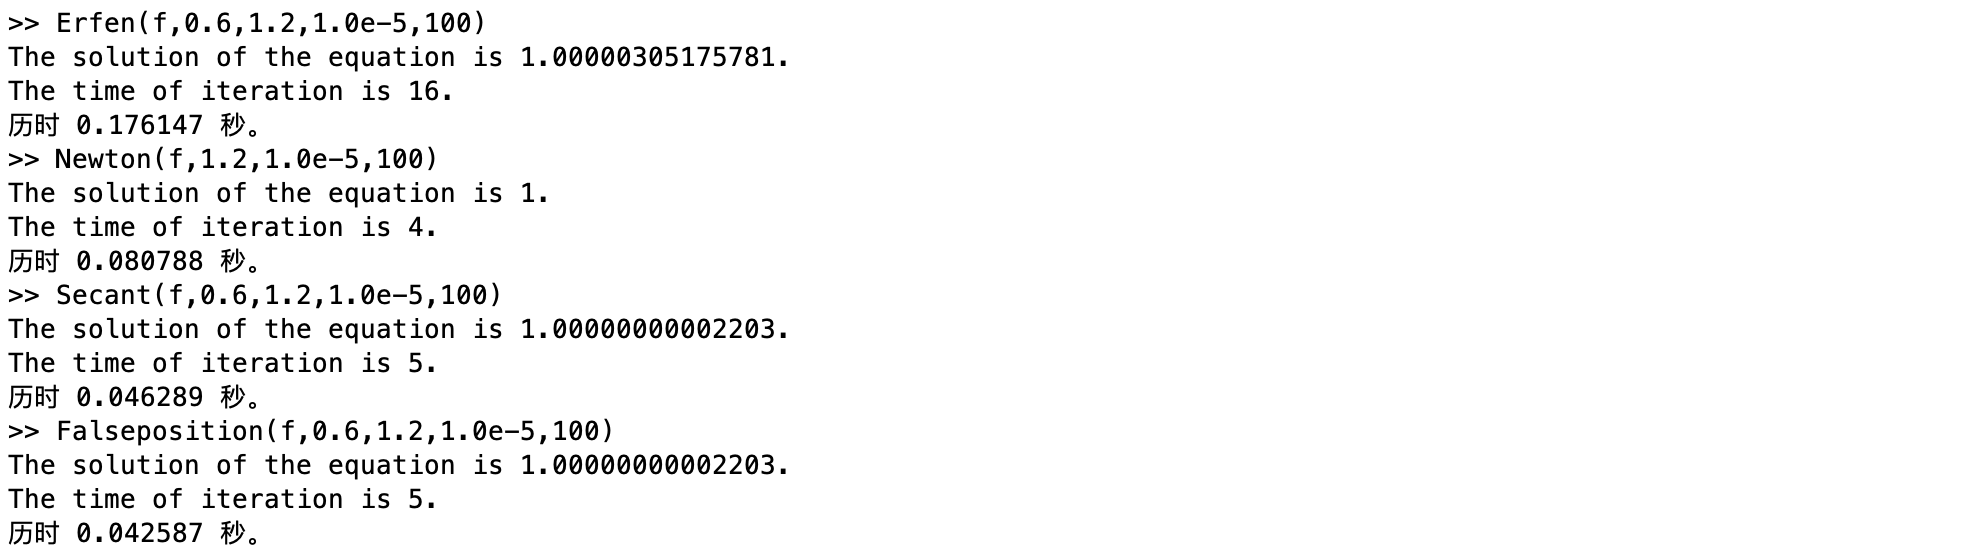
\includegraphics[scale=0.5]{运行程序2.jpg}
    \end{figure}

    发现除二分法正常运行(效率较低,迭代次数为16次),牛顿法,割线法均以极少次数与CPU时间迭代到$p=1$。因此下面再看一个例子主要观察下面三者的区别。

\subsection{2.2 求解含正弦函数的方程在0.48周围的根}

    下面考虑另一个方程(2.3节习题14)
    $$f(x)=tan(\pi x)-6=0
    $$
    在0.48周围(注意:0.5点处趋向于无穷取不到)的一个零点取值为$arctan(6)/\pi\approx0.447431543288747$。下图是该方程在$[0,0.5)$之间的图像:
    \begin{figure}[h]
    \centering
    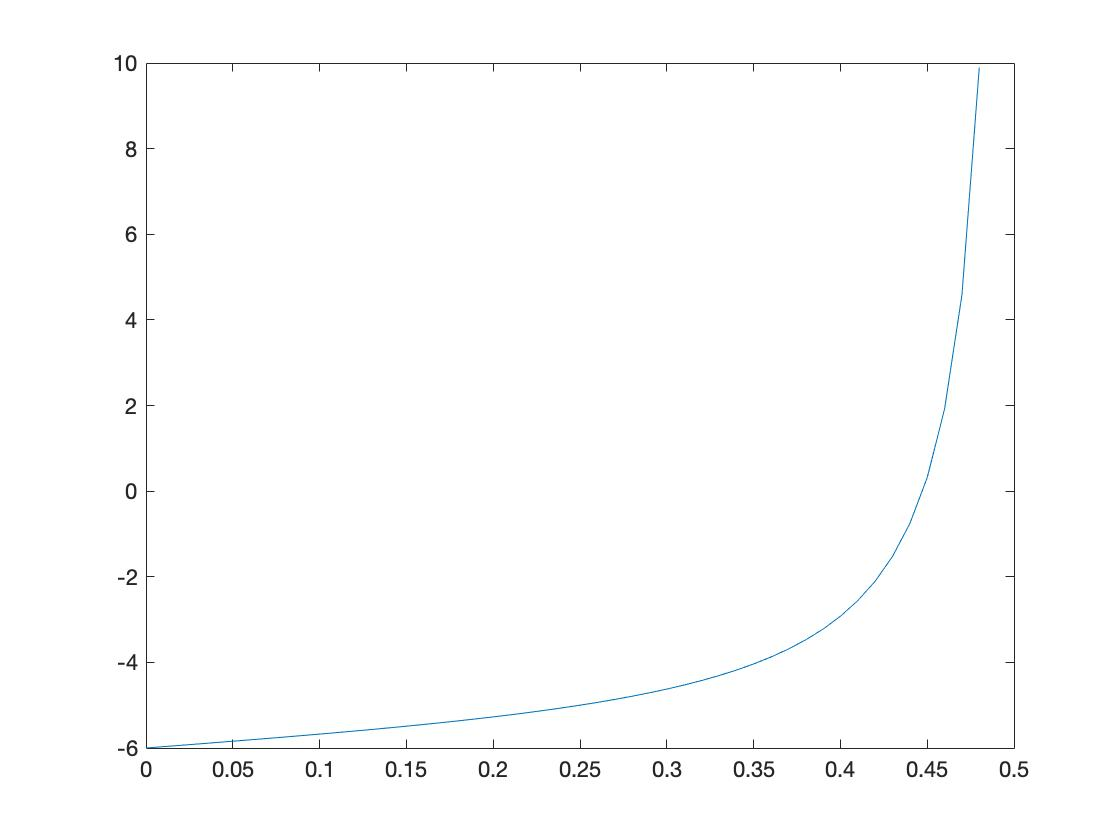
\includegraphics[scale=0.19]{第二个函数.jpg}
    \caption{含正弦函数的方程图像}
    \label{含正弦函数的方程图像}
    \end{figure}

    再下面是分别运行二分法,牛顿法,割线法与试位法的程序,如下所示:
    \begin{figure}[h]
    \centering
    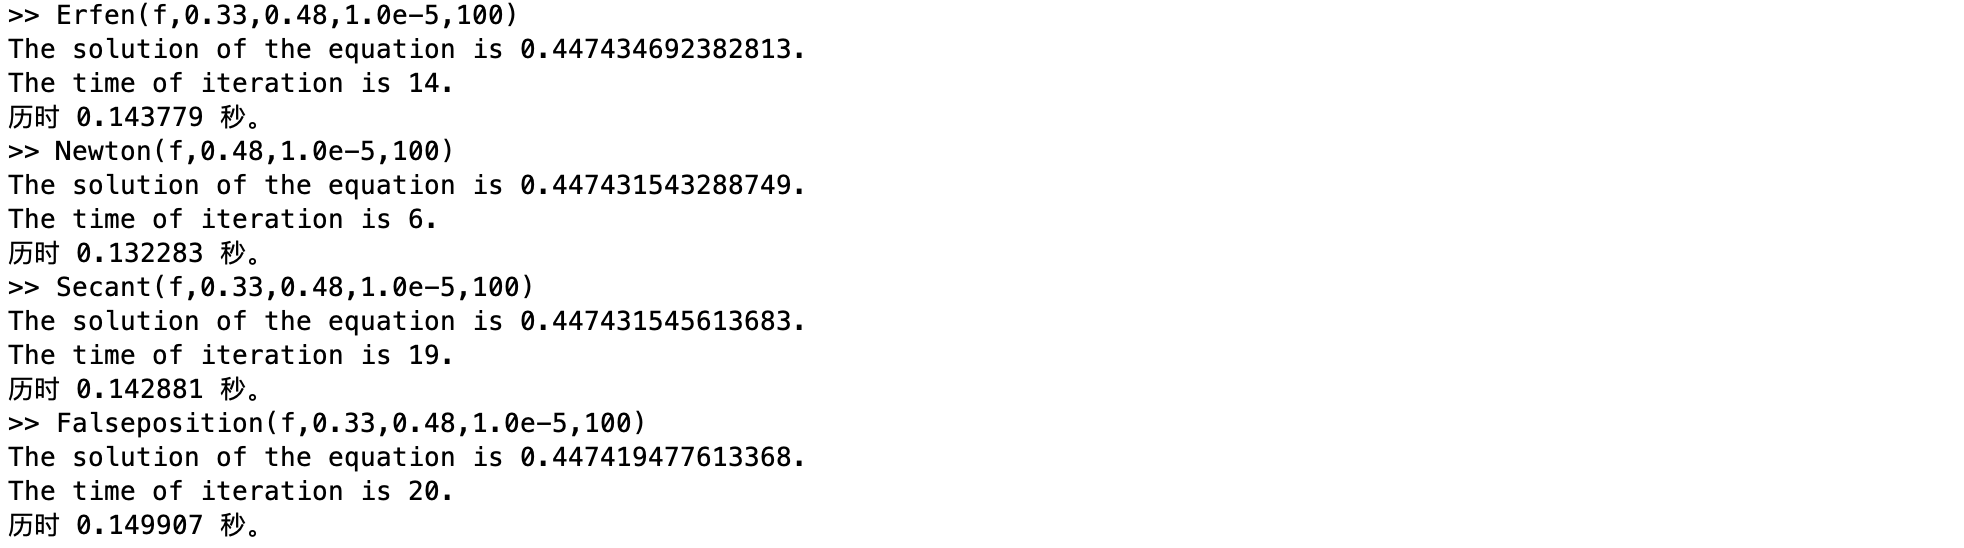
\includegraphics[scale=0.5]{运行程序3.jpg}
    \end{figure}

    结果发现,所有程序都照常运行迭代到所求根的附近。重点观察牛顿法与割线法:牛顿法迭代次数(6次)相对于割线法迭代次数(19次)较少,意即割线法比牛顿法收敛速度慢一点;但牛顿法CPU运行时间(0.132283秒)相对于割线法CPU运行时间(0.142881秒)所差无几,这似乎令人费解。细想可知牛顿法每次都要计算导数值,而割线法每次仅需计算函数值,故每次迭代的计算量较小。因此这两种方法可以说各有所长:\textbf{牛顿法迭代次数较少而割线法迭代计算量较小。因此分析具体函数时应考察函数导数的复杂度。}最后,割线法与试位法所有数据近乎一致,但\textbf{试位法需要初始值不同号的前提},否则算法运行结果几乎是错误的。

    然后对比误差精度,所有方程都达到要求的误差,关键对比牛顿法与割线法发现,牛顿法的精度($10^{-14}$级)远超割线法的精度($10^{-8}$级)。因此,\textbf{牛顿法在同样误差精度的要求下,迭代次数不仅少同时精度同时远大于割线法的精度。}

\subsection{2.3 求解含正弦函数方程的迭代过程分析}

    最后,我们利用Matlab生成牛顿法,割线法迭代过程(表格),如下所示:
    \begin{figure}[h]
    \centering
    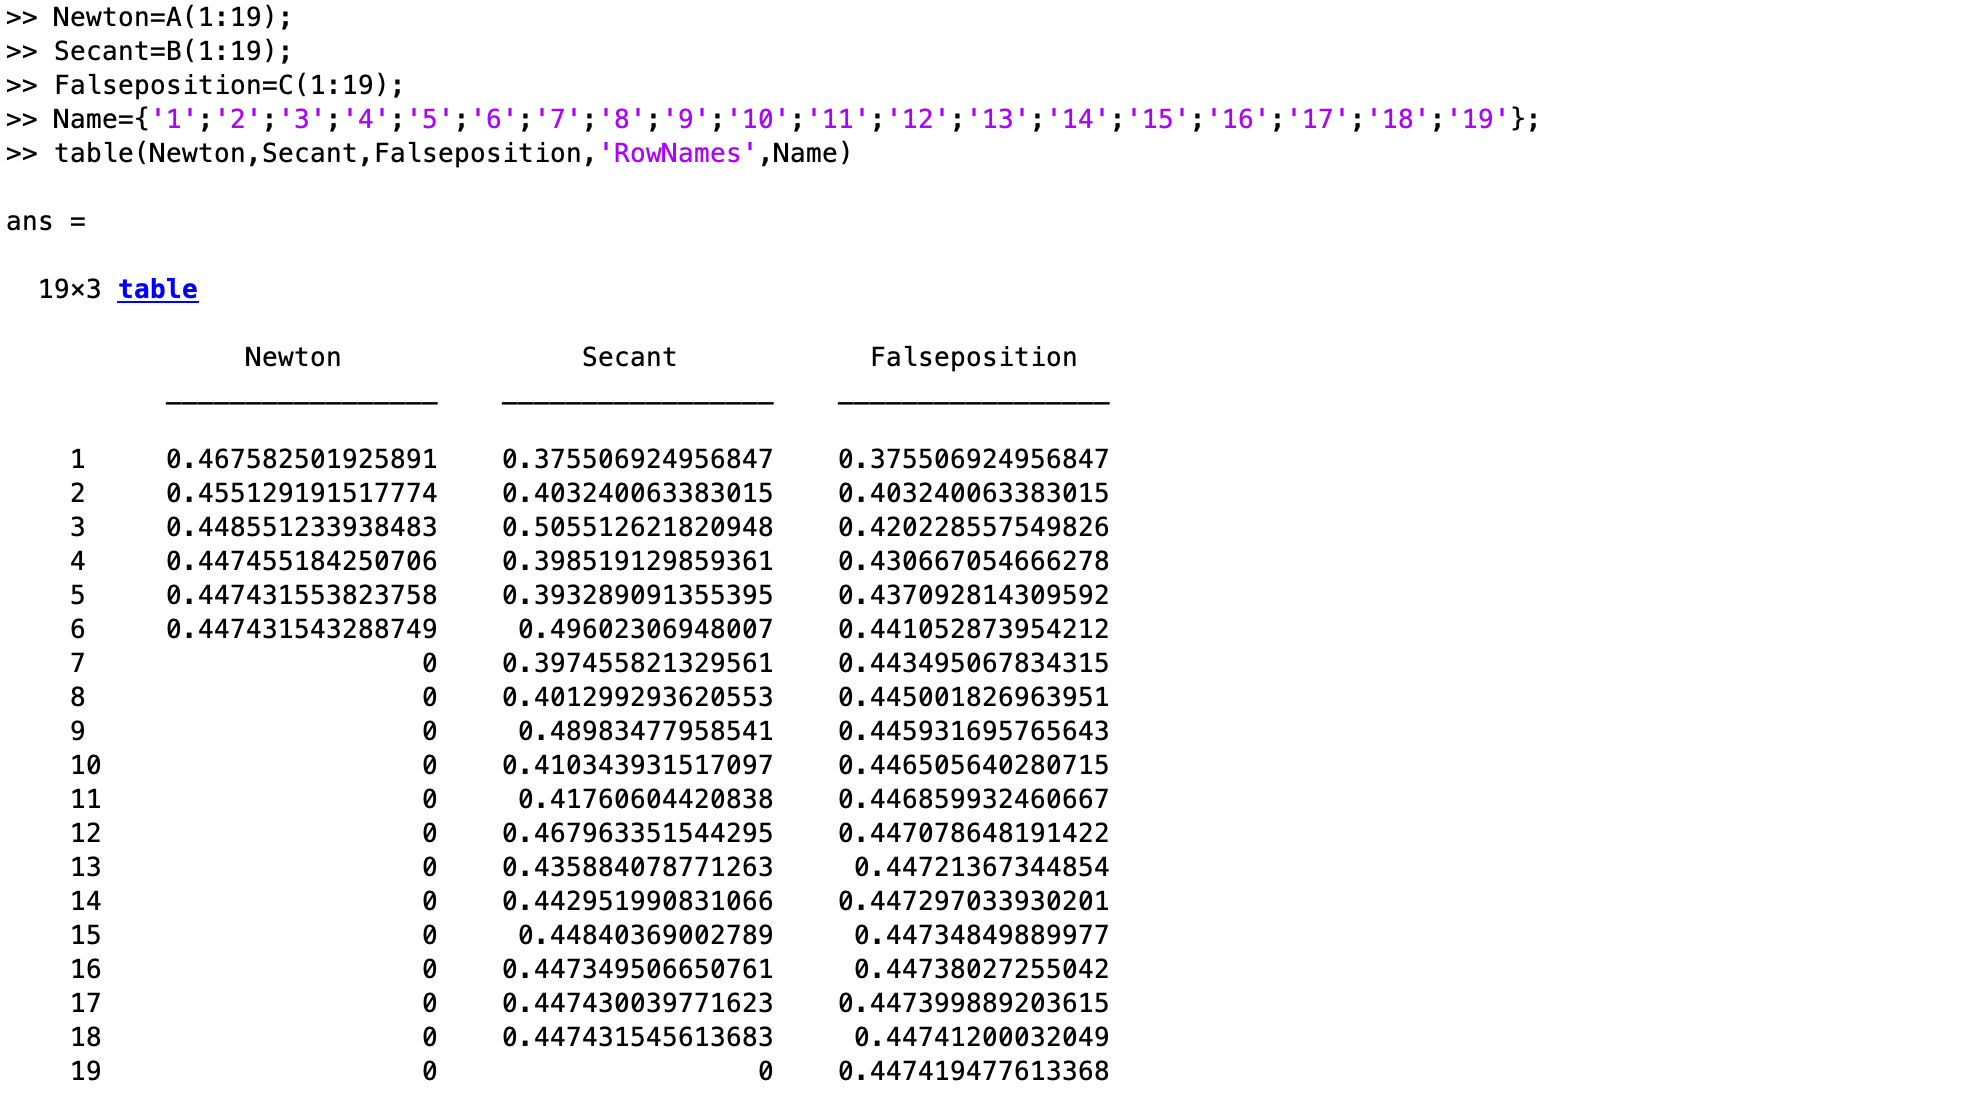
\includegraphics[scale=0.5]{Eq2_NSF_Table.jpg}
    \end{figure}

    但对比效果不明显,因此画出折线图对比。如下所示为图像。

    分析显示:牛顿法可以平稳逼近零点,割线法波动较大,试错法较平稳但收敛速度与割线法持平。

    \begin{figure}[h]
    \centering
    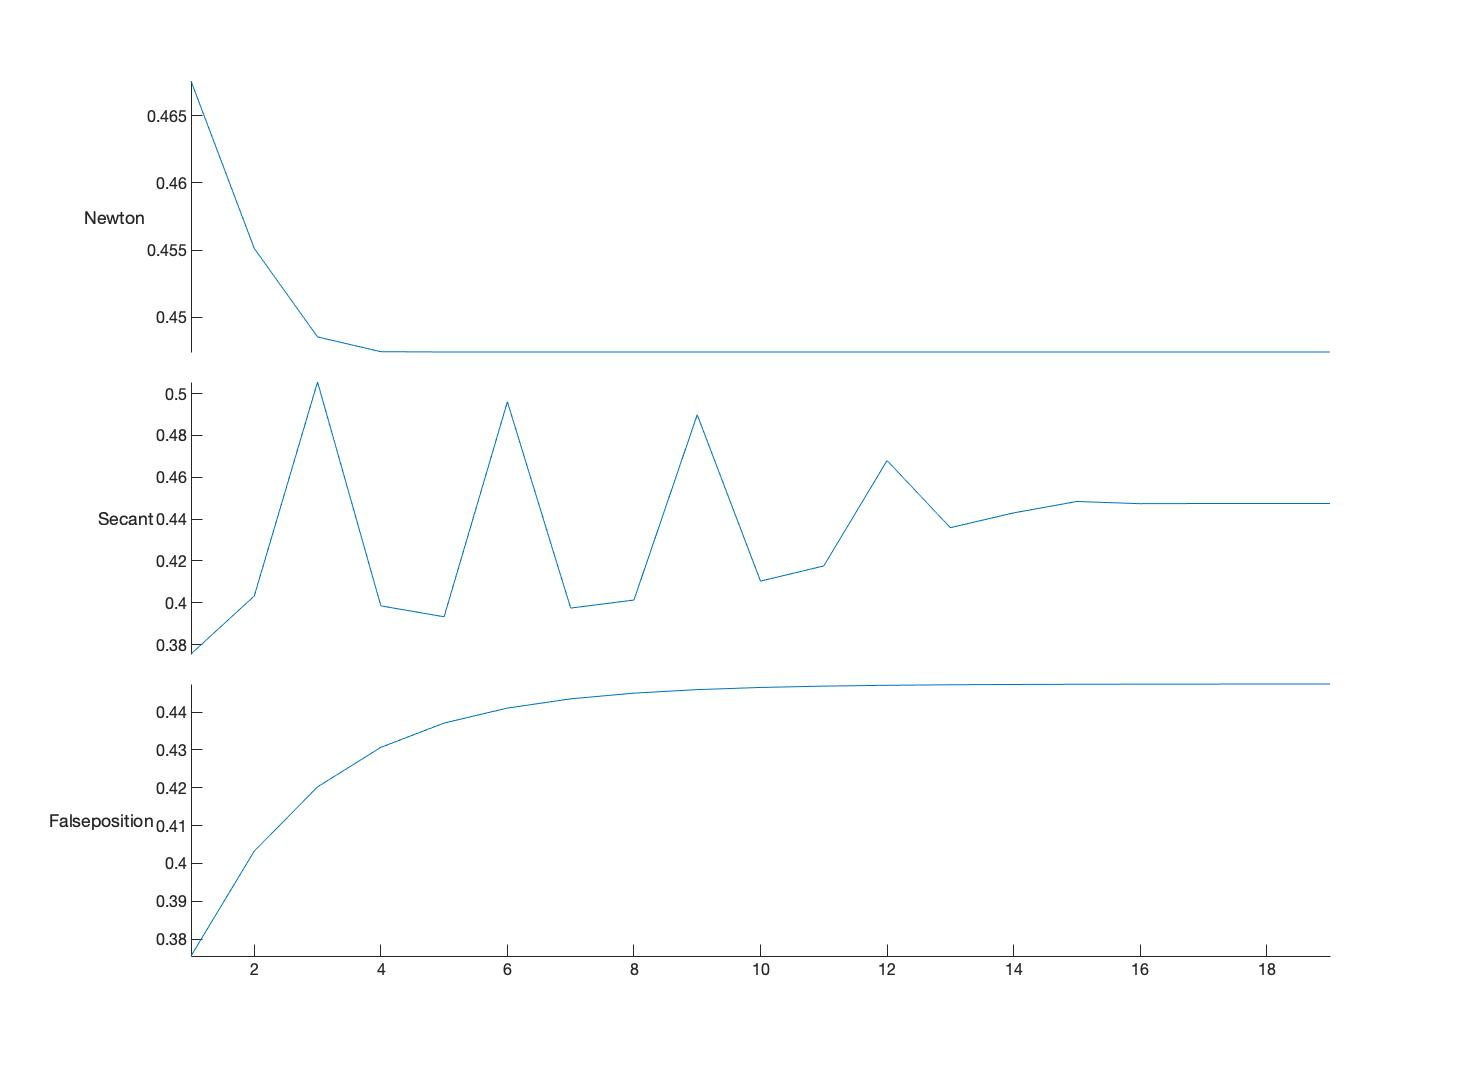
\includegraphics[scale=0.1712]{Eq2_NSF.jpg}
    \caption{求解第二个方程中牛顿法,割线法,试错法的折线图}
    \label{求解第二个方程中牛顿法,割线法,试错法的折线图}
    \end{figure}


\newpage

\section{3. 不动点迭代与Steffensen迭代对比}

\subsection{3.1 不动点迭代与Steffensen迭代求解三阶 Legendre 方程}

    依上面所示,牛顿法,割线法与试位法对$P_3(x)=0$在1.2附近的根均有较好的效果,现在转用不动点法求解。通过令$g(x):=P_3(x)+x$将方程求根转化为不动点迭代$g(x)=x$。则下面分别运行不动点迭代与Steffensen迭代的程序,并将初始点(宽松地)设置为1.4。如下所示:
    \begin{figure}[h]
    \centering
    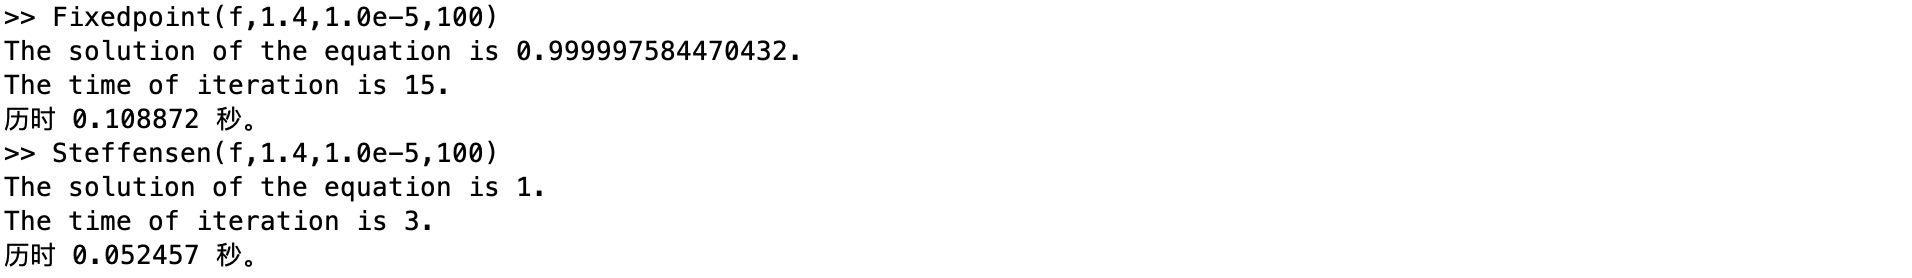
\includegraphics[scale=0.5]{运行程序.jpg}
    \end{figure}

    发现上述计算结果都满足在误差范围内,其中不动点迭代的误差计算如下
    $$\bigg|\frac{p_{15}-p}{p}\bigg|=2.415529568\times 10^{-6}.
    $$
    发现不动点迭代的关键位数(Significant Digit)为6位而Steffensen迭代计算结果完全精准!同时不动点迭代需要的迭代次数为15次,而Steffensen迭代的迭代次数仅为3次。在计算机CPU时间上,不动点迭代为0.060890 秒,而Steffensen迭代的迭代次数仅为0.223619 秒。经过其他方程的验证,二者差别同样明显。\textbf{这说明在一定条件下,由于Steffensen迭代为二阶收敛,加速后的Steffensen迭代相比于不动点迭代更优。}

\subsection{3.2 求解三阶 Legendre 方程的迭代过程分析}

    最后我们分析二分法,牛顿法,割线法,试位法,不动点迭代与Steffensen迭代在求解三阶 Legendre 方程的迭代过程。同2.3节,实现如下:

    \begin{figure}[h]
    \centering
    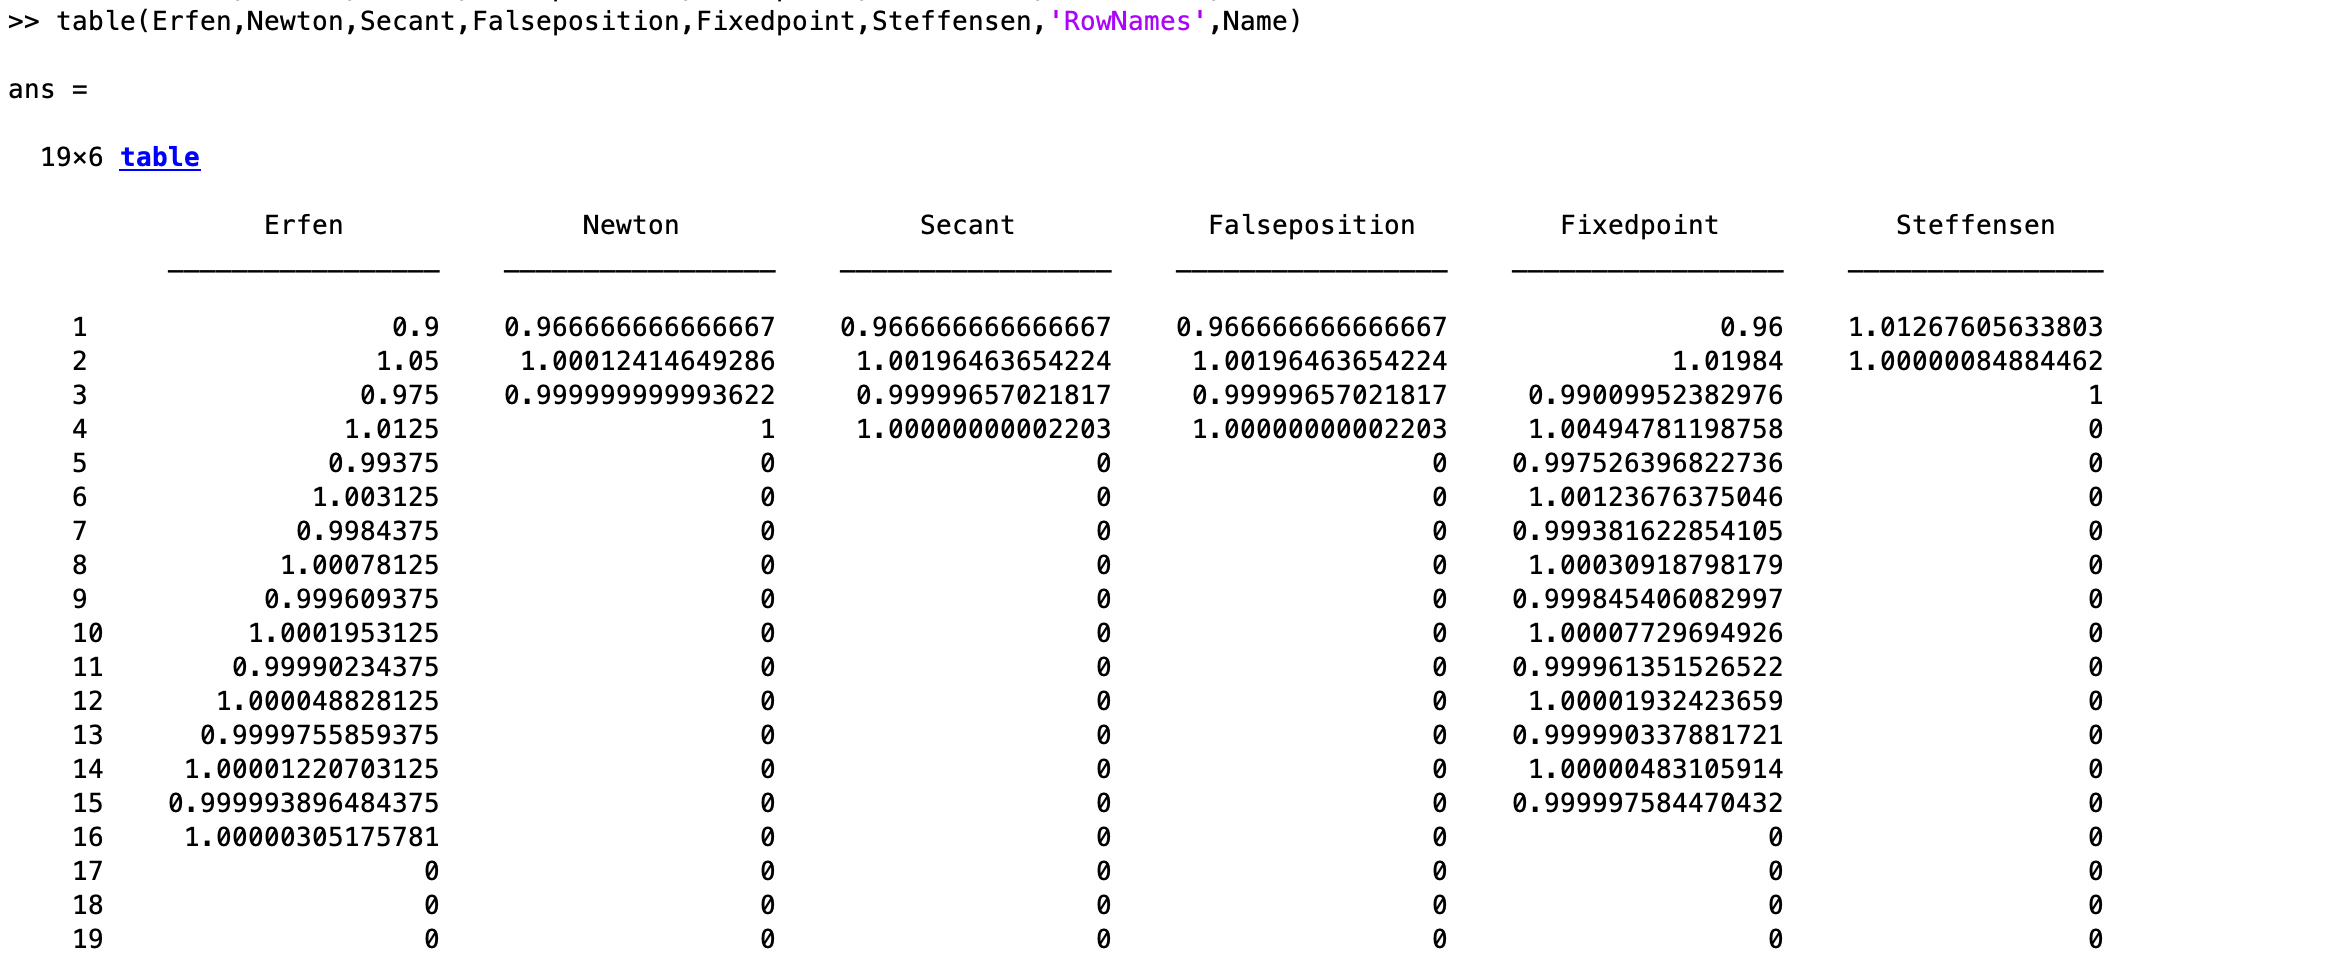
\includegraphics[scale=0.4]{Eq1_ENSFFS_Table.jpg}
    \end{figure}

    同样,绘制折线图对比。如下所示为图像。

    \begin{figure}[h]
    \centering
    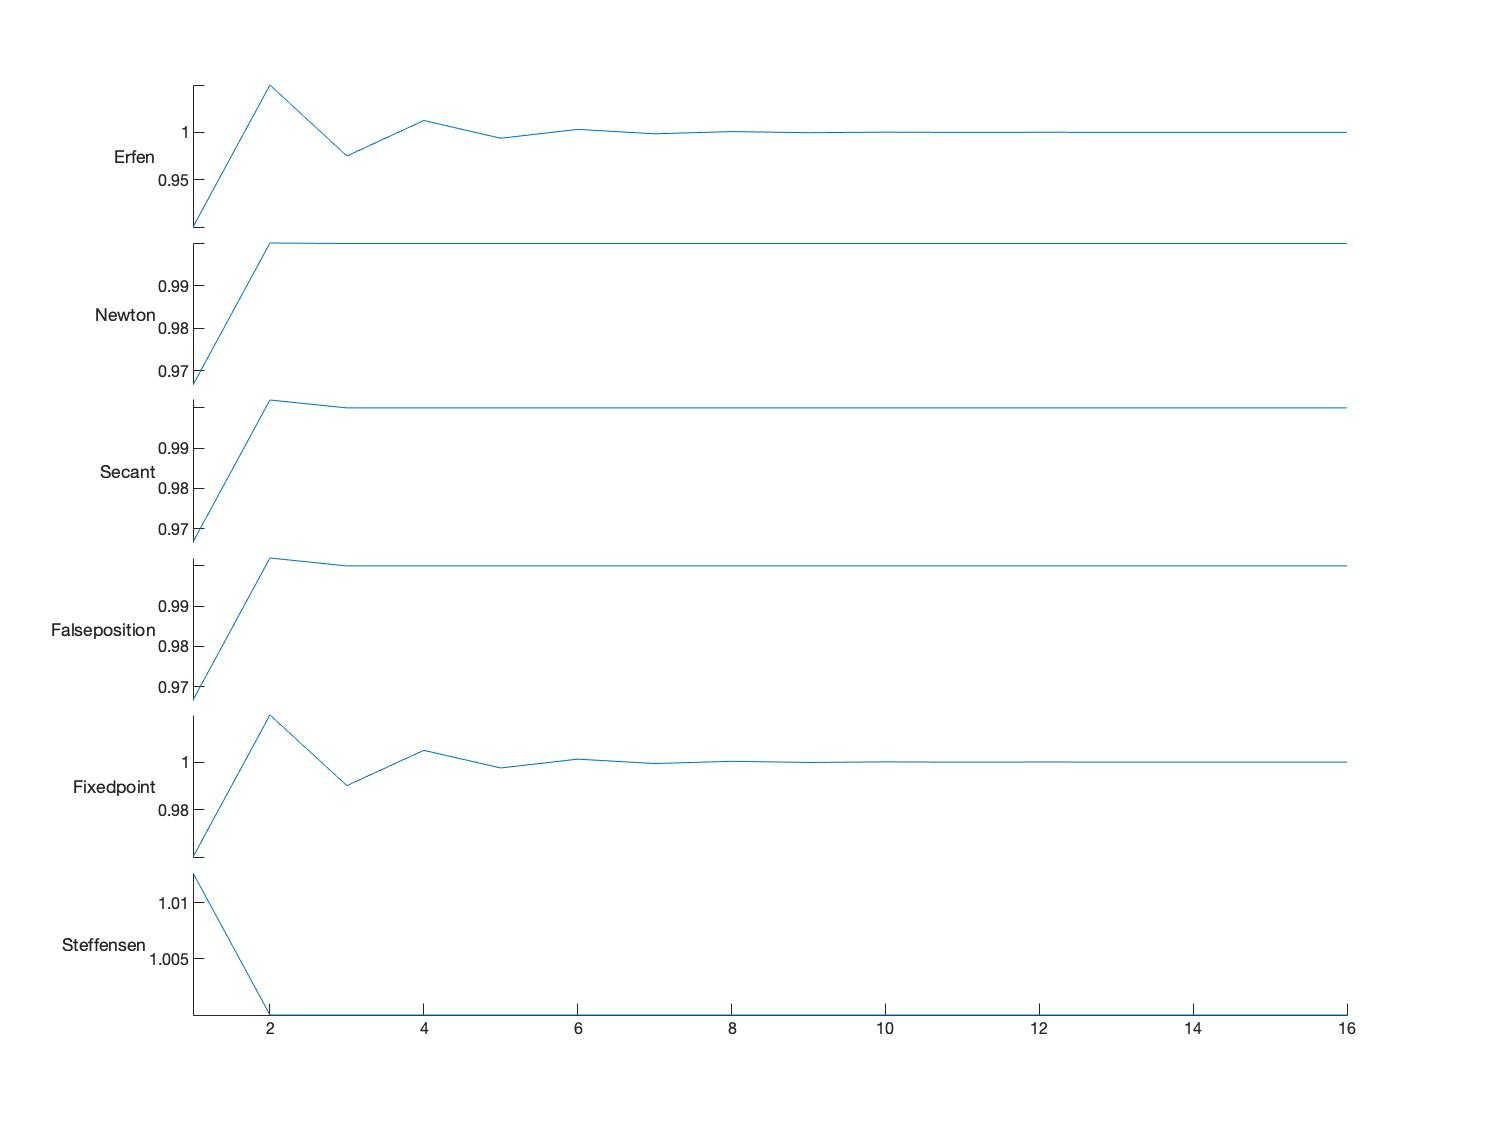
\includegraphics[scale=0.18]{Eq1_ENSFFS.jpg}
    \end{figure}

    分析显示:二分法表现平稳,在大幅度波动8次后便趋向于平稳;牛顿法在3次迭代后直接平稳达到精确值;割线法与试位法迭代次数稍多于牛顿法且精确度稍逊于牛顿法;不动点迭代表现与二分法一致,表现平稳;加速后的Steffensen迭代表现与牛顿法一样好在3次迭代后平稳达到精确值。

\section{4. 多项式中的Horner与Muller算法}
    首先是Horner算法,即\textbf{采用嵌套方式}去计算多项式在固定点的值与导数值。例如$P(x)=x^2+x$在x=1处的函数值与导数值分别为2,3。如下所示:
    \begin{figure}[h]
    \centering
    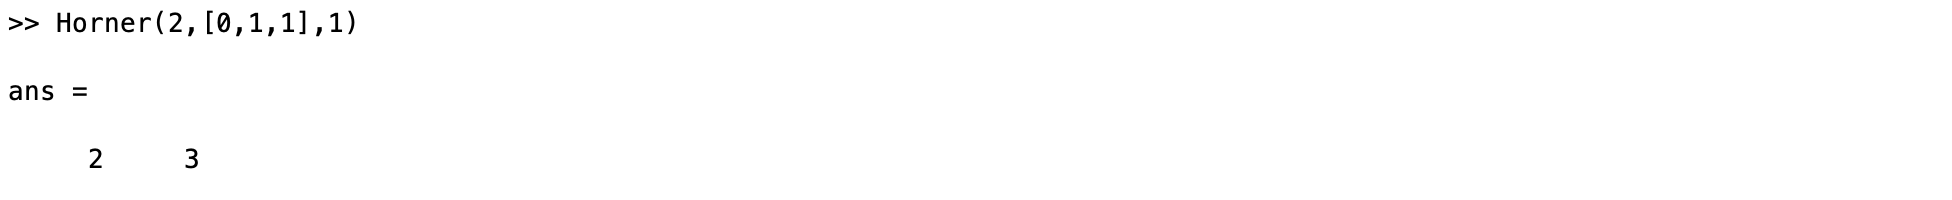
\includegraphics[scale=0.5]{运行程序4.jpg}
    \end{figure}

    其次是Muller算法的一个简单应用:求解$x^2+1=0$的复根。如下所示:

    \begin{figure}[h]
    \centering
    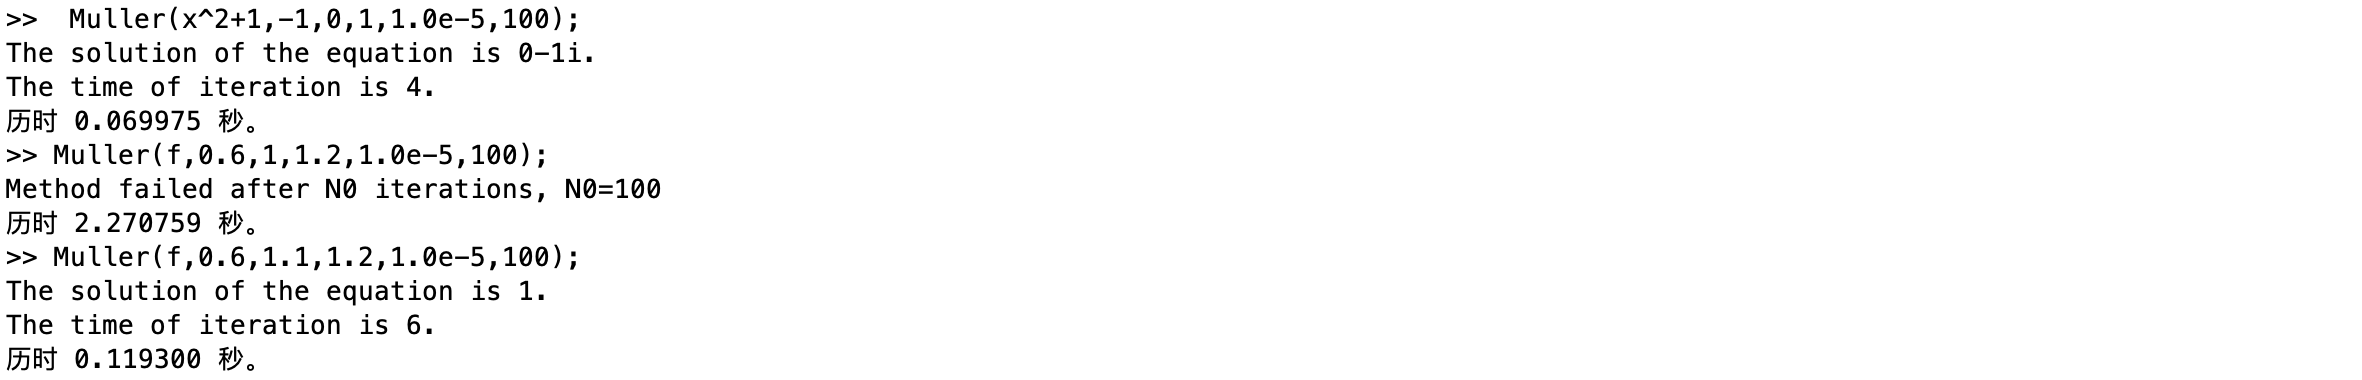
\includegraphics[scale=0.5]{运行程序5.jpg}
    \end{figure}

    之后还是回归到求解三阶Legendre方程在1.2附近的根,观察与之前的算法在迭代次数及CPU运行时间上的对比。利用Muller算法求解三阶Legendre方程,代码在上方实现。

    发现,如初始点不在零点取值,则算法在这个多项式方程上表现很优:首先迭代次数仅为6次就达到精度要求,同时\textbf{在同一个方程求根问题中历时在所有算法中几乎最短},且最终结果的关键位数为12,计算如下:
    $$\bigg|\frac{p_{6}-p}{p}\bigg|=1.511\times 10^{-12}<5\times 10^{-12}
    $$

\newpage

\section{5. 代码附录}
    \subsection{5.1 二分法}
    \begin{lstlisting}
    % Bisection method for a solution of f(x)=0
    function output=Erfen(f,a,b,TOL,N0)
    % Calculate runtime of the program
    tic;
    % If TOL is missing,error is assumed to be the standard one 1E-3.
    if(nargin==4)
        TOL=1.0e-3;
    end 
    % Initialize variable for iteration ordinal number 
    i=1;
    FA=subs(f,a);
    k=1;
    J=zeros(1,100);
    while (i<=N0)
        p=a+(b-a)/2;
        FP=subs(f,p);
        J(k)=p; % show the process of iteration
        k=k+1;
        if ((FP==0)||((b-a)/2<TOL))
            disp(['The solution of the equation is ',num2str(p,15),'.']);
            disp(['The time of iteration is ',num2str(i),'.']);
            output=J;
            toc
            return;
        end
        i=i+1;
        if(FA*FP>0)
            a=p; 
            FA=FP;
        else 
            b=p;
        end
    end
    % the procedure was unsuccessful
    disp(['Method failed after N0 iterations, N0=',num2str(N0)])
    toc
    \end{lstlisting}


    \subsection{5.2 不动点迭代法}
    \begin{lstlisting}
    % Fixed point itteration for a solution to p=g(p)
    function output=Fixedpoint(g,p0,TOL,N0)
    % Calculate runtime of the program
    tic;
    % If TOL is missing,error is assumed to be the standard error 1E-3.
    if(nargin==3)
        TOL=1.0e-3;
    end 
    % Initialize variable for iteration ordinal number 
    i=1;
    k=1;
    J=zeros(1,100); 
    while (i<=N0)
        p=subs(g,p0);
        p=double(p);
        J(k)=p; % show the process of iteration
        k=k+1;
        if (abs(p-p0)<TOL)
            disp(['The solution of the equation is ',num2str(p,15),'.']);
            disp(['The time of iteration is ',num2str(i),'.']);
            output=J;
            toc
            return;
        end
        i=i+1;
        p0=p;
    end
    % the procedure was unsuccessful
    disp(['Method failed after N0 iterations, N0=',num2str(N0)])
    toc
    \end{lstlisting}

    \subsection{5.3 Muller法}
    \begin{lstlisting}
        % Muller's method for a solution of f(x)=0
    function output=Muller(f,x0,x1,x2,TOL,N0)
    % Calculate runtime of the program
    tic;
    % If TOL is missing,error is assumed to be the standard one 1E-3.
    if(nargin==4)
        TOL=1.0e-3;
    end 
    % Initialize variable for iteration ordinal number 
    i=3;
    h1=x1-x0;
    h2=x2-x1;
    fx0=subs(f,x0);
    fx0=double(fx0);
    fx1=subs(f,x1);
    fx1=double(fx1);
    fx2=subs(f,x2);
    fx2=double(fx2);
    d1=(fx1-fx0)/h1;
    d2=(fx2-fx1)/h2;
    d=(d2-d1)/(h2+h1);
    k=1;
    J=zeros(1,100);
    while (i<=N0)
        b=d2+h2*d;
        D=(b^2-4*fx2*d)^(1/2);
        if (abs(b-D)<abs(b+D))
            E=b+D;
        else
            E=b-D;
        end
        h=-2*fx2/E;
        p=x2+h;
        J(k)=p; % show the process of iteration
        k=k+1;
        if (abs(h)<TOL)
            disp(['The solution of the equation is ',num2str(p),'.']);
            disp(['The time of iteration is ',num2str(i),'.']);
            output=J;
            toc
            return;
        end
        i=i+1;
        x0=x1;
        x1=x2;
        x2=p;
        h1=x1-x0;
        h2=x2-x1;
        fx0=subs(f,x0);
        fx0=double(fx0);
        fx1=subs(f,x1);
        fx1=double(fx1);
        fx2=subs(f,x2);
        fx2=double(fx2);
        d1=(fx1-fx0)/h1;
        d2=(fx2-fx1)/h2;
        d=(d2-d1)/(h2+h1);
    end
    % the procedure was unsuccessful
    disp(['Method failed after N0 iterations, N0=',num2str(N0)])
    toc
    \end{lstlisting}

    \subsection{5.4 牛顿法}
    \begin{lstlisting}
        % Newton's method for a solution to f(x)=0
    function output=Newton(f,p0,TOL,N0)
    % Calculate runtime of the program
    tic;
    % If TOL is missing,error is assumed to be the standard error 1E-3.
    if(nargin==3)
        TOL=1.0e-3;
    end 
    % Initialize variable for iteration ordinal number 
    i=1;
    k=1;
    J=zeros(1,100);
    while (i<=N0)
        fx=subs(f,p0);
        fx=double(fx);
        df=diff(f);
        df=subs(df,p0);
        df=double(df);
        p=p0-fx/df;
        J(k)=p; % show the process of iteration
        k=k+1;
        if (abs(p-p0)<TOL)
            disp(['The solution of the equation is ',num2str(p,15),'.']);
            disp(['The time of iteration is ',num2str(i),'.']);
            output=J;
            toc
            return;
        end
        i=i+1;
        p0=p;
    end
    % the procedure was unsuccessful
    disp(['Method failed after N0 iterations, N0=',num2str(N0)])
    toc
    \end{lstlisting}

    \subsection{5.5 试错法}
    \begin{lstlisting}
        % Method of False position for a solution to f(x)=0
    function output=Falseposition(f,p0,p1,TOL,N0)
    % Calculate runtime of the program
    tic;
    % If TOL is missing,error is assumed to be the standard error 1E-3.
    if(nargin==3)
        TOL=1.0e-3;
    end 

    % Initialize variable for iteration ordinal number 
    i=2;
    q0=subs(f,p0);
    q0=double(q0);
    q1=subs(f,p1);
    q1=double(q1);
    k=1;
    J=zeros(1,100);
    while (i<=N0)
        p=p1-q1*(p1-p0)/(q1-q0);
        J(k)=p; % show the process of iteration
        k=k+1;
        if (abs(p-p1)<TOL)
            disp(['The solution of the equation is ',num2str(p,15),'.']);
            disp(['The time of iteration is ',num2str(i),'.']);
            output=J;
            toc
            return;
        end
        i=i+1; %update p0,q0,p1,q1.
        q=subs(f,p);
        q=double(q);
        if (q*q1<0)
            p0=p1;
            q0=q1;
        end
        p1=p;  %update p1,q1.
        q1=q;
    end
    % the procedure was unsuccessful
    disp(['Method failed after N0 iterations, N0=',num2str(N0)])
    toc
    \end{lstlisting}

    \subsection{5.6 Horner法}
    \begin{lstlisting}
    % Horner's method to evaluate a polynomial and its derivative at x0
    function output=Horner(n,a,x0)
    % compute cofficient b(n) for P and b(n-1) for Q
    y=a(n+1);
    z=a(n+1);
    for j=n-1:1
        y=x0*y+a(j+1); % compute b(j) for P
        z=x0*z+y;  % compute b(j-1) for Q
    end
    y=x0*y+a(1);% compute b(0) for P
    output=[y,z];
    \end{lstlisting}

    \subsection{5.7 割线法}
    \begin{lstlisting}
    % Secant method for a solution to f(x)=0
    function output=Secant(f,p0,p1,TOL,N0)
    % Calculate runtime of the program
    tic;
    % If TOL is missing,error is assumed to be the standard error 1E-3.
    if(nargin==3)
        TOL=1.0e-3;
    end 
    % Initialize variable for iteration ordinal number 
    i=2;
    q0=subs(f,p0);
    q0=double(q0);
    q1=subs(f,p1);
    q1=double(q1);
    k=1;
    J=zeros(1,100);
    while (i<=N0)
        p=p1-q1*(p1-p0)/(q1-q0);
        J(k)=p; % show the process of iteration
        k=k+1;
        if (abs(p-p1)<TOL)
            disp(['The solution of the equation is ',num2str(p,15),'.']);
            disp(['The time of iteration is ',num2str(i),'.']);
            output=J;
            toc
            return;
        end
        i=i+1; 
        p0=p1; % update p0,q0,p1,q1
        q0=q1;
        p1=p;
        q1=subs(f,p);
        q1=double(q1);
    end
    % the procedure was unsuccessful
    disp(['Method failed after N0 iterations, N0=',num2str(N0)])
    toc
    \end{lstlisting}

    \subsection{5.8 Steffensen法}
    \begin{lstlisting}
    % Steffensen's method for a solution to p=g(p)
    function output=Steffensen(g,p0,TOL,N0)
    % Calculate runtime of the program
    tic;
    % If TOL is missing,error is assumed to be the standard error 1E-3.
    if(nargin==3)
        TOL=1.0e-3;
    end 
    % Initialize variable for iteration ordinal number 
    i=1;
    k=1;
    J=zeros(1,100);
    while (i<=N0)
        p1=subs(g,p0);
        p1=double(p1);
        p2=subs(g,p1);
        p2=double(p2);
        p=p0-(p1-p0)*(p1-p0)/(p2-2*p1+p0);
        J(k)=p; % show the process of iteration
        k=k+1;
        if (abs(p-p0)<TOL)
            disp(['The solution of the equation is ',num2str(p,15),'.']);
            disp(['The time of iteration is ',num2str(i),'.']);
            output=J;
            toc
            return;
        end
        i=i+1; 
        p0=p;
    end
    % the procedure was unsuccessful
    disp(['Method failed after N0 iterations, N0=',num2str(N0)])
    toc
    \end{lstlisting}

\end{document}
